\begin{evenBlock}{Get the Snitch}

\begin{minipage}[t]{\linewidth}
    \centering
    
    \begin{minipage}{.5\linewidth} % Left column and width
        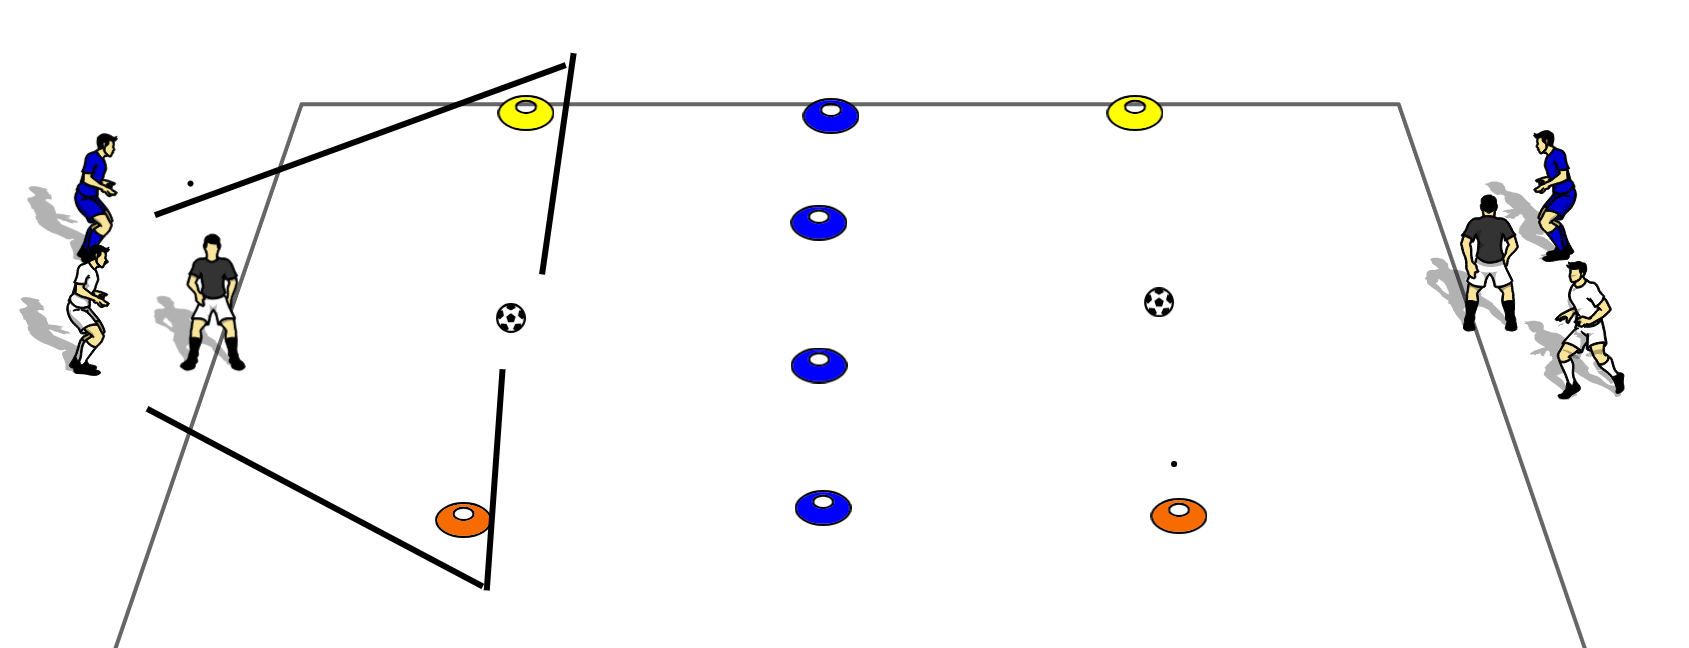
\includegraphics[width=\textwidth]{../img/Trimmed/Get_the_Snitch}
    \end{minipage}
    \hspace{0.05\linewidth}
    \begin{minipage}{.4\linewidth} % Left column and width
        \textbf{Drill Description:}
        The object is to get the ball (the snitch) and take it across the opposite end line.
        \begin{enumerate}
            \setlength{\itemsep}{0pt}
            \setlength{\parskip}{0pt}
            \setlength{\parsep}{0pt}
            \item Coach calls go and kicks a ball into the field, both players race around their cone to get to the ball.
            \item First player to get the ball tries to drive across the fair end line while the other player defends that line.
        \end{enumerate}
    \end{minipage}
\end{minipage}
\vspace{12pt}

%\textbf{Coaching Points:}
%\begin{itemize}
%    \setlength{\itemsep}{0pt}
%    \setlength{\parskip}{0pt}
%    \setlength{\parsep}{0pt}
%    \item Explain marking a player is to remain within 2 or 3 feet of the attacking player.
%    \item Explain how to mark a player goal side (defender between the attacker and goal).
%    \item Attackers try to lose their marks by passing.
%\end{itemize}
\end{evenBlock}